\documentclass{standalone}
\usepackage{tikz}
\usetikzlibrary{patterns, positioning}


\begin{document}
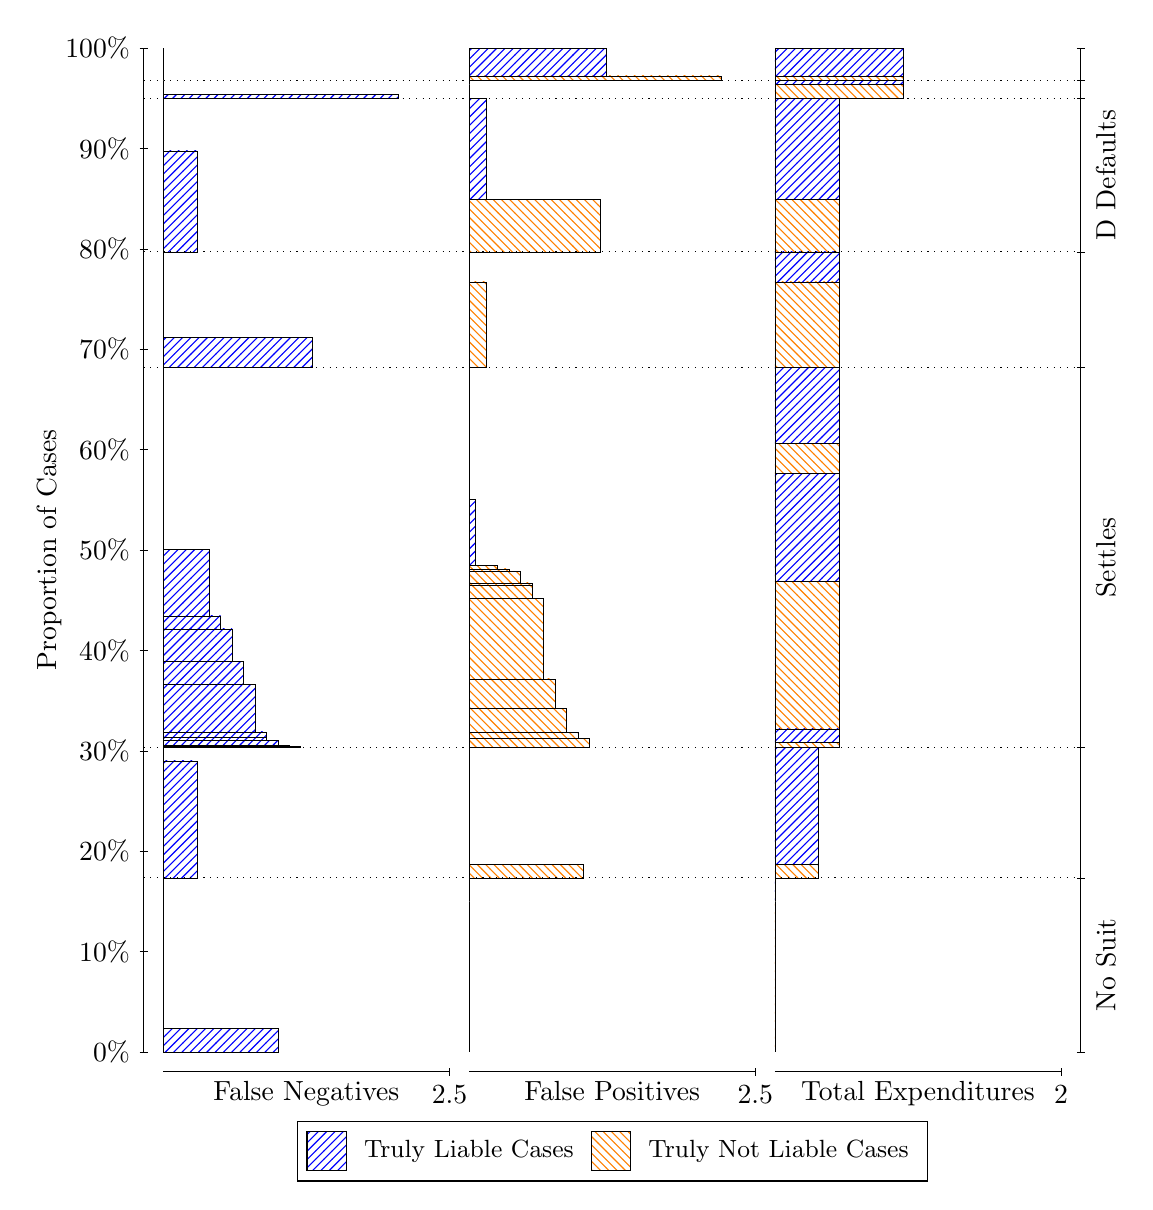
\begin{tikzpicture}
\draw[black, very thin] (1.5,1.75) -- (1.5,14.5);
\node[rotate=90, text=black, anchor=center] at (0.3, 8.125) {Proportion of Cases};
\draw[black, very thin] (1.45,1.75) -- (1.55,1.75);
\node[text=black, anchor=east] at (1.45, 1.75) {0\%};
\draw[black, very thin] (1.45,3.025) -- (1.55,3.025);
\node[text=black, anchor=east] at (1.45, 3.025) {10\%};
\draw[black, very thin] (1.45,4.3) -- (1.55,4.3);
\node[text=black, anchor=east] at (1.45, 4.3) {20\%};
\draw[black, very thin] (1.45,5.575) -- (1.55,5.575);
\node[text=black, anchor=east] at (1.45, 5.575) {30\%};
\draw[black, very thin] (1.45,6.85) -- (1.55,6.85);
\node[text=black, anchor=east] at (1.45, 6.85) {40\%};
\draw[black, very thin] (1.45,8.125) -- (1.55,8.125);
\node[text=black, anchor=east] at (1.45, 8.125) {50\%};
\draw[black, very thin] (1.45,9.4) -- (1.55,9.4);
\node[text=black, anchor=east] at (1.45, 9.4) {60\%};
\draw[black, very thin] (1.45,10.675) -- (1.55,10.675);
\node[text=black, anchor=east] at (1.45, 10.675) {70\%};
\draw[black, very thin] (1.45,11.95) -- (1.55,11.95);
\node[text=black, anchor=east] at (1.45, 11.95) {80\%};
\draw[black, very thin] (1.45,13.225) -- (1.55,13.225);
\node[text=black, anchor=east] at (1.45, 13.225) {90\%};
\draw[black, very thin] (1.45,14.5) -- (1.55,14.5);
\node[text=black, anchor=east] at (1.45, 14.5) {100\%};

\draw[black, very thin] (13.4,1.75) -- (13.4,14.5);
\draw[black, very thin] (13.35,1.75) -- (13.45,1.75);
\node[anchor=west] at (13.35, 1.75) {};
\draw[black, very thin] (13.35,3.9623) -- (13.45,3.9623);
\node[anchor=west] at (13.35, 3.9623) {};
\draw[black, very thin] (13.35,5.6152) -- (13.45,5.6152);
\node[anchor=west] at (13.35, 5.6152) {};
\draw[black, very thin] (13.35,10.446) -- (13.45,10.446);
\node[anchor=west] at (13.35, 10.446) {};
\draw[black, very thin] (13.35,11.911) -- (13.45,11.911);
\node[anchor=west] at (13.35, 11.911) {};
\draw[black, very thin] (13.35,13.858) -- (13.45,13.858);
\node[anchor=west] at (13.35, 13.858) {};
\draw[black, very thin] (13.35,14.09) -- (13.45,14.09);
\node[anchor=west] at (13.35, 14.09) {};
\draw[black, very thin] (13.35,14.5) -- (13.45,14.5);
\node[anchor=west] at (13.35, 14.5) {};

\draw[black, very thin, pattern color=blue, pattern=north east lines] (1.75,1.75) rectangle (3.2033,2.0504);
\draw[black, very thin, pattern color=orange, pattern=north west lines] (1.75,2.0504) rectangle (1.75,3.9623);
\draw[black, very thin, pattern color=blue, pattern=north east lines] (1.75,3.9623) rectangle (2.186,5.4473);
\draw[black, very thin, pattern color=orange, pattern=north west lines] (1.75,5.4473) rectangle (1.75,5.6152);
\draw[black, very thin, pattern color=blue, pattern=north east lines] (1.75,5.6152) rectangle (3.494,5.6284);
\draw[black, very thin, pattern color=blue, pattern=north east lines] (1.75,5.6284) rectangle (3.3487,5.6405);
\draw[black, very thin, pattern color=blue, pattern=north east lines] (1.75,5.6405) rectangle (3.2033,5.7114);
\draw[black, very thin, pattern color=blue, pattern=north east lines] (1.75,5.7114) rectangle (3.058,5.741);
\draw[black, very thin, pattern color=blue, pattern=north east lines] (1.75,5.741) rectangle (3.058,5.814);
\draw[black, very thin, pattern color=blue, pattern=north east lines] (1.75,5.814) rectangle (2.9127,6.4142);
\draw[black, very thin, pattern color=blue, pattern=north east lines] (1.75,6.4142) rectangle (2.7673,6.7082);
\draw[black, very thin, pattern color=blue, pattern=north east lines] (1.75,6.7082) rectangle (2.622,7.1222);
\draw[black, very thin, pattern color=blue, pattern=north east lines] (1.75,7.1222) rectangle (2.4767,7.2886);
\draw[black, very thin, pattern color=blue, pattern=north east lines] (1.75,7.2886) rectangle (2.3313,8.1335);
\draw[black, very thin, pattern color=orange, pattern=north west lines] (1.75,8.1335) rectangle (1.75,10.446);
\draw[black, very thin, pattern color=blue, pattern=north east lines] (1.75,10.446) rectangle (3.6393,10.827);
\draw[black, very thin, pattern color=orange, pattern=north west lines] (1.75,10.827) rectangle (1.75,11.911);
\draw[black, very thin, pattern color=blue, pattern=north east lines] (1.75,11.911) rectangle (2.186,13.193);
\draw[black, very thin, pattern color=orange, pattern=north west lines] (1.75,13.193) rectangle (1.75,13.858);
\draw[black, very thin, pattern color=blue, pattern=north east lines] (1.75,13.858) rectangle (4.7293,13.913);
\draw[black, very thin, pattern color=orange, pattern=north west lines] (1.75,13.913) rectangle (1.75,14.09);
\draw[black, very thin, pattern color=orange, pattern=north west lines] (1.75,14.09) rectangle (1.75,14.147);
\draw[black, very thin, pattern color=blue, pattern=north east lines] (1.75,14.147) rectangle (1.75,14.5);
\draw[black, very thin, pattern color=orange, pattern=north west lines] (5.6333,1.75) rectangle (5.6333,3.6619);
\draw[black, very thin, pattern color=blue, pattern=north east lines] (5.6333,3.6619) rectangle (5.6333,3.9623);
\draw[black, very thin, pattern color=orange, pattern=north west lines] (5.6333,3.9623) rectangle (7.0867,4.1301);
\draw[black, very thin, pattern color=blue, pattern=north east lines] (5.6333,4.1301) rectangle (5.6333,5.6152);
\draw[black, very thin, pattern color=orange, pattern=north west lines] (5.6333,5.6152) rectangle (7.1593,5.7364);
\draw[black, very thin, pattern color=orange, pattern=north west lines] (5.6333,5.7364) rectangle (7.014,5.8069);
\draw[black, very thin, pattern color=orange, pattern=north west lines] (5.6333,5.8069) rectangle (6.8687,6.1133);
\draw[black, very thin, pattern color=orange, pattern=north west lines] (5.6333,6.1133) rectangle (6.7233,6.4894);
\draw[black, very thin, pattern color=orange, pattern=north west lines] (5.6333,6.4894) rectangle (6.578,7.5125);
\draw[black, very thin, pattern color=orange, pattern=north west lines] (5.6333,7.5125) rectangle (6.4327,7.6765);
\draw[black, very thin, pattern color=orange, pattern=north west lines] (5.6333,7.6765) rectangle (6.4327,7.7085);
\draw[black, very thin, pattern color=orange, pattern=north west lines] (5.6333,7.7085) rectangle (6.2873,7.8548);
\draw[black, very thin, pattern color=orange, pattern=north west lines] (5.6333,7.8548) rectangle (6.142,7.8845);
\draw[black, very thin, pattern color=orange, pattern=north west lines] (5.6333,7.8845) rectangle (5.9967,7.9276);
\draw[black, very thin, pattern color=blue, pattern=north east lines] (5.6333,7.9276) rectangle (5.706,8.7725);
\draw[black, very thin, pattern color=blue, pattern=north east lines] (5.6333,8.7725) rectangle (5.6333,10.446);
\draw[black, very thin, pattern color=orange, pattern=north west lines] (5.6333,10.446) rectangle (5.8513,11.531);
\draw[black, very thin, pattern color=blue, pattern=north east lines] (5.6333,11.531) rectangle (5.6333,11.911);
\draw[black, very thin, pattern color=orange, pattern=north west lines] (5.6333,11.911) rectangle (7.3047,12.576);
\draw[black, very thin, pattern color=blue, pattern=north east lines] (5.6333,12.576) rectangle (5.8513,13.858);
\draw[black, very thin, pattern color=orange, pattern=north west lines] (5.6333,13.858) rectangle (5.6333,14.034);
\draw[black, very thin, pattern color=blue, pattern=north east lines] (5.6333,14.034) rectangle (5.6333,14.09);
\draw[black, very thin, pattern color=orange, pattern=north west lines] (5.6333,14.09) rectangle (8.8307,14.147);
\draw[black, very thin, pattern color=blue, pattern=north east lines] (5.6333,14.147) rectangle (7.3773,14.5);
\draw[black, very thin, pattern color=orange, pattern=north west lines] (9.5167,1.75) rectangle (9.5167,3.6619);
\draw[black, very thin, pattern color=blue, pattern=north east lines] (9.5167,3.6619) rectangle (9.5167,3.9623);
\draw[black, very thin, pattern color=orange, pattern=north west lines] (9.5167,3.9623) rectangle (10.062,4.1301);
\draw[black, very thin, pattern color=blue, pattern=north east lines] (9.5167,4.1301) rectangle (10.062,5.6152);
\draw[black, very thin, pattern color=orange, pattern=north west lines] (9.5167,5.6152) rectangle (10.334,5.6857);
\draw[black, very thin, pattern color=blue, pattern=north east lines] (9.5167,5.6857) rectangle (10.334,5.8521);
\draw[black, very thin, pattern color=orange, pattern=north west lines] (9.5167,5.8521) rectangle (10.334,7.7217);
\draw[black, very thin, pattern color=blue, pattern=north east lines] (9.5167,7.7217) rectangle (10.334,9.1029);
\draw[black, very thin, pattern color=orange, pattern=north west lines] (9.5167,9.1029) rectangle (10.334,9.4752);
\draw[black, very thin, pattern color=blue, pattern=north east lines] (9.5167,9.4752) rectangle (10.334,10.446);
\draw[black, very thin, pattern color=orange, pattern=north west lines] (9.5167,10.446) rectangle (10.334,11.531);
\draw[black, very thin, pattern color=blue, pattern=north east lines] (9.5167,11.531) rectangle (10.334,11.911);
\draw[black, very thin, pattern color=orange, pattern=north west lines] (9.5167,11.911) rectangle (10.334,12.576);
\draw[black, very thin, pattern color=blue, pattern=north east lines] (9.5167,12.576) rectangle (10.334,13.858);
\draw[black, very thin, pattern color=orange, pattern=north west lines] (9.5167,13.858) rectangle (11.152,14.034);
\draw[black, very thin, pattern color=blue, pattern=north east lines] (9.5167,14.034) rectangle (11.152,14.09);
\draw[black, very thin, pattern color=orange, pattern=north west lines] (9.5167,14.09) rectangle (11.152,14.147);
\draw[black, very thin, pattern color=blue, pattern=north east lines] (9.5167,14.147) rectangle (11.152,14.5);
\draw[black, dotted] (1.5,3.9623) -- (13.4,3.9623);
\draw[black, dotted] (1.5,5.6152) -- (13.4,5.6152);
\draw[black, dotted] (1.5,10.446) -- (13.4,10.446);
\draw[black, dotted] (1.5,11.911) -- (13.4,11.911);
\draw[black, dotted] (1.5,13.858) -- (13.4,13.858);
\draw[black, dotted] (1.5,14.09) -- (13.4,14.09);
\draw[black, very thin] (1.75,1.5) -- (5.3833,1.5);
\node[text=black, anchor=north] at (3.5667, 1.5) {False Negatives};
\draw[black, very thin] (5.3833,1.45) -- (5.3833,1.55);
\node[text=black, anchor=north] at (5.3833, 1.45) {2.5};

\draw[black, very thin] (5.6333,1.5) -- (9.2667,1.5);
\node[text=black, anchor=north] at (7.45, 1.5) {False Positives};
\draw[black, very thin] (9.2667,1.45) -- (9.2667,1.55);
\node[text=black, anchor=north] at (9.2667, 1.45) {2.5};

\draw[black, very thin] (9.5167,1.5) -- (13.15,1.5);
\node[text=black, anchor=north] at (11.333, 1.5) {Total Expenditures};
\draw[black, very thin] (13.15,1.45) -- (13.15,1.55);
\node[text=black, anchor=north] at (13.15, 1.45) {2};

\node[text=black, centered, rotate=90] at (13.72, 2.8561) {No Suit};

\node[text=black, centered, rotate=90] at (13.72, 8.0306) {Settles};

\node[text=black, centered, rotate=90] at (13.72, 12.884) {D Defaults};



\draw (7.449999999999999,1.5) node[draw=none] (baseCoordinate) {};
\begin{scope}[align=center]
        \matrix[scale=0.5, draw=black, below=0.5cm of baseCoordinate, nodes={draw}, column sep=0.1cm]{
            \node[rectangle, draw, minimum width=0.5cm, minimum height=0.5cm, pattern color=blue, pattern=north east lines] {}; &
            \node[draw=none, font=\small, text=black] (B) {Truly Liable Cases}; &
            \node[rectangle, draw, minimum width=0.5cm, minimum height=0.5cm, pattern color=orange, pattern=north west lines] {}; &
            \node[draw=none, font=\small, text=black] (B) {Truly Not Liable Cases}; \\
            };
\end{scope}

\end{tikzpicture}
\end{document}